\documentclass{article}
\usepackage[utf8]{inputenc}

\usepackage{amssymb, amsmath, lmodern, units, icomma, color, graphicx, bbm, hyperref, pdfpages, csquotes, listings, subcaption, epstopdf}

\usepackage{caption}
\usepackage{blindtext}
\usepackage[inline]{enumitem}
\usepackage{minted}
\usemintedstyle{friendly}
\graphicspath{ {../Images/} }
%\usepackage{xcolor}

\setlength{\parindent}{0em}
\setlength{\parskip}{0.5em}

\title{Avsnitt 1 \\
\large Om komplexa tal, Eulers formel, signaler, grundläggande implementering och annat mysigt}
\author{ }
\date{}

\begin{document}

\maketitle

\section{Komplexa tal med DSL}
Då inleder vi med komplexa tal! Det här är något som antagligen känns ganska
hemvant för de flesta av er men vi tar och repeterar lite ändå och passar på
att visa hur man kan implementera ämnet med DSL.

Imaginära tal. Var kommer dom ifrån tänker ni? Jo, det är så att om man
försökte dra roten ur ett negativt tal så blev det jobbigt, fram till att
någon introducerade imaginära tal. Som är jobbiga på sitt eget sätt istället.
Så därför bestämdes det att $\sqrt{-1}$ ska vara \emph{i}.

Som tur är så är det hela ganska konsekvent utformat så att $\sqrt{-2}$ också
blir $\sqrt{2}i$, och $\sqrt{-3}$ blir $\sqrt{3} i$. Så om man tar roten ur
vilken negativt tal som helst så får man samma svar som det positiva fallet
fast med ett i med.

Vi kommer dock inte använda oss av beteckningen \emph{i} i våra texter, eftersom
att man inom fysik, elektronik och flera andra ämnen redan använder bokstaven i
för att beteckna en ström. Därfor brukar man ofta använda j inom signallära
istället, för att undvika missförstånd, och det kommer vi också göra.
%Alltså kan man skriva så här: känns lite överflödigt men jag sätter dit den om gruppen vill.

Komplexa tal kan ses som ett par utav reella värden, där första
värdet i talet är reellt och det andra värdet är den imaginära
delen. Det kan dock vara så att en eller båda av dessa delar är noll.
T.ex. $7+0*j$ blir ju bara 7.


\textbf{Kryssfråga 1:} Vad är den reela delen av $10 + 5 j$
\begin{enumerate}[label={\alph*)},font={\bfseries}]
\item 5
\item 10
\end{enumerate}
\textbf{Kryssfråga 2:} Vad är den imaginära delen i talet $4 + \frac{6}{5}j$?
\begin{enumerate}[label={\alph*)},font={\bfseries}]
\item 4
\item $\frac{6}{5}$
\end{enumerate}

Att skriva
\begin{minted}{haskell}
Complex 13 37
\end{minted}
i vårt DSL är samma sak som att skriva 13 + 37j, där 13 är reellt och 37 är imaginärt. Det är alltså inget ‘j’ i vårt DSL som indikerar att det är imaginärt utan man måste bara skriva dem i rätt ordning. Det ser som tur liknande ut i matten så det är ganska lätt att komma ihåg! %Sista meningen är lite konstig.

Nu betraktar vi det komplexa talet $13+37j$.
Vi döper detta till \emph{leet} så att vi slipper skriva ut alltihop i framtiden.
\begin{minted}{haskell}
leet = Complex 13 37
\end{minted}
Om du nu känner att du vill veta vad det reella talet i paret är,
då kan man skriva en funktion realPart som bara ger dig den reella delen.
\begin{minted}{haskell}
realPart :: Complex -> Double
realPart (Complex c) = fst c
\end{minted}
Då kan vi enkelt få fram den reella delen av \emph{leet} genom\\
\begin{minted}{haskell}
realPart (leet)
\end{minted}
vilket ger oss svaret 13.
Se så enkelt det blev!
Så för att få ut den imaginära delen av talet så gör vi en funktion imPart.

\textbf{Övning 1:} Definiera en funktion imPart som ger imaginärdelen av ett komplext tal.
Denna funktion bör ge: $imPart (leet) = 37$

\textbf{Övning 2:} Om vi nu skulle vilja skriva ut talet på vanligt mattespråk så skulle vi kunna göra en funktion som kan heta $printComplex$. Här får du ett kodskelett för en sådan funktion. Fyll i det som saknas.
\begin{minted}{haskell}
printComplex :: Complex -> String
printComplex z
  | r == 0 = show im ++ "j"
  | im == 0 = ...
  | otherwise = ...
    where im = imPart z
          r = realPart z
\end{minted}
Om vi då kör
\begin{minted}{haskell}
printComplex 5 12
\end{minted}
får vi:
\begin{minted}{haskell}
5 + 12j
\end{minted}
Och
\begin{minted}{haskell}
printComplex (leet)
\end{minted}
ger oss:
\begin{minted}{haskell}
13 + 37j
\end{minted}

Hur skulle man då göra för att faktiskt räkna på detta?
Då måste man definiera hur matematiska tecken ska tolkas när man arbetar med
komplexa tal.

Addition för komplexa tal är ganska lätt om ni kommer ihåg det.
Om man är reell bryr man sig bara om andra reella tal, och vice versa för
imaginära tal.

\textbf{Övning 3:} Här får du ett kodskelett för addition med komplexa tal.
Fyll i det som ska stå i parentesen.
\begin{minted}{haskell}
instance Num Complex where
    z + w           = Complex (...)
\end{minted}
\textbf{Test:} Vad får man om man \underline{adderar} $10 + 5j$ med $2 -1j$?
Bekräfta med programmet.

Multiplikation blir lite krångligare.
Om vi multiplicerar två komplexa tal, vi kallar dem z och w, ser det ut såhär:
\begin{minted}{haskell}
    z * w           = Complex (realZ*realW - imZ*imW,
                                realZ*imW + realW*imZ)
        where realZ = realPart z
                   realW = realPart w
                   imZ   = imPart z
                   imW   = imPart w
\end{minted}
Vilket då blir samma sak som:
$$z \; w = (Re(Z) * Re(W) - Im(Z)*Im(W)) + (Re(Z)*Im(W) + Re(W)*Im(Z))j$$
\textbf{Test:} Vad får man om man \underline{multiplicerar} $10 + 5j$ med $2 -1j$?
Bekräfta med programmet.

Det kan även vara bra att ha en funktion som negerar ett komplext tal.
T.ex. $13+37j$ ska då alltså bli $-13-37j$

\textbf{Övning 4:} Här är ett kodskellet till funktionen negate.
Fyll i det som ska stå i parentesen.
\begin{minted}{haskell}
negate z        = Complex (...)
\end{minted}
Absolutbeloppet på ett komplext tal kan man räkna ut på samma sätt som man
räknar ut hypotenusan i en rätvinklig triangel.

\textbf{Övning 5:} Här är ett kodskelett till en funktion som ger absolutbeloppet
av ett komplext tal. Fyll i det som saknas.
\begin{minted}{haskell}
    abs z           = Complex (hyp, 0)
        where hyp   = ...
              r      = realPart z
              im   = imPart z
\end{minted}
\textbf{Test:} Vad är absolutbeloppet av $6 + 3j$? Bekräfta med programmet.

\textbf{Test:} Hur skriver man ut heltalet 5 som ett komplext tal?
Bekräfta med programmet (fromInteger).

\section{Eulers formel}
Eulers formel, eller Enigmatic Euler's Formula som den också kallas,
är en formel för att skriva om komplexa tal från en exponentiell funktion
till trigonometriska funktioner och tvärtom.

Är det någon som verkligen vet hur trigonometiska funktioner funkar?
Förmodligen..., men det skulle väl inte skada om det fanns ett sätt att skriva
om trigonometiska funktioner till komplexa tal och tvärtom. Här kommer Eulers formel in!
$$e^{jt} = cos(t) + jsin(t) $$
\textbf{Kryssfråga 3:} Vad blir $e^{3jt}$ omskrivet med Eulers formel?
\begin{enumerate}[label={\alph*)},font={\bfseries}]
\item $3 \cos(t) + 3 j \sin(t)$
\item $\cos(3t) + j \sin(3t)$
\item $\cos(t) + j \sin(t) + 3 t$
\end{enumerate}

\textbf{Kryssfråga 4:} Vad blir $\cos(4t)+j \sin(4t)+5$ omskrivet med Eulers formel?
\begin{enumerate}[label={\alph*)},font={\bfseries}]
\item $e^{j4+5}$
\item $5e^{j4}$
\item $e^{j4} + 5$
\end{enumerate}

Med lite magiska omskrivningar kan man bryta ut cosinus respektive sinus ur formeln
vilket ger följande funktioner.
$$cos(t) = (e^{jt} + e^{-jt})/2 $$
$$sin(t) = (e^{jt} - e^{-jt})/(2j) $$
Varför skulle flera komponenter vara bättre då? Det tar vi upp i avsnitt 3
om Fourierserier! Men nu vet ni hur man gör!

\section{Signaler}

Då har vi kommit fram till signaler! Signaler kan i praktiken vara lite allt
möjligt som t.ex. ljud, elektrisk ström, dataströmmar, mm. Men ur ett
matematiskt perspektiv är en signal ingenting annat än en funktion som beror
av tid, eller någon annan variabel. Om detta sedan är en funktion som
beskriver ljudstyrka eller antalet prickar på en vägg struntar vi i. Vi kan
räkna på dem på samma sätt oavsett om det gäller prickar eller ljud.


\subsection{Diskreta och kontinuerliga signaler}

Man kan säga att det finns två grundtyper av signaler, kontinuerliga och
diskreta. Vad menar man då med detta? Jo, en signal kallas kontinuerlig om
den är beroende av en kontinuerlig variabel. Denna variabel är oftast tid,
men inte nödvändigtvis. Om funktionen istället har en diskret variabel kallar
man den för en diskret signal. Denna diskreta variabel är ofta, men inte
alltid, heltal. Det där var ju logiskt och bra, nu ska vi bara reda ut vad
som menas med kontinuerliga och diskreta variabler.

Att en variabel är kontinuerlig innebär att den har ett oändligt antal värden
även om det bara är definierad i ett visst intervall. Om vi t.ex. betecknar
tiden mellan kl 14:00 och 15:00 med variabeln t så har den ett oändligt antal
möjliga värden i intervallet $14 < t < 15$. Variabeln t kan då t.ex. anta
värdet $14.6$, men den kan också anta värdet $14.6000000001$. Det finns helt
enkelt ingen gräns för hur många värden t kan anta, även om intervallet är
begränsat.

Här kan du se ett exempel på en kontinuerlig funktion, $f(t)=2t$
\begin{figure}[ht]
\centerline{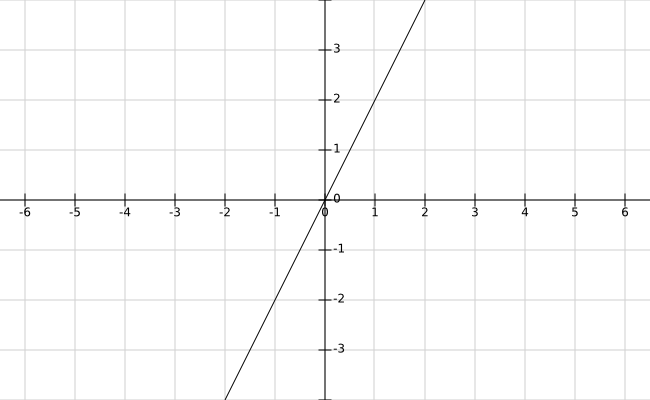
\includegraphics[scale=0.55]{image06}}
\caption{}
\label{}
\end{figure}
\newpage
En diskret variabel däremot har bara ett visst antal värden den kan anta och
en diskret funktion är bara definierad för dessa möjliga värden. Om vi t.ex.
beteckar alla heltal med variabeln n så kommer en funktion $f[n]$ vara
definierad, alltså ha ett värde, i punkten $f[2]$ men vara odefinierad, sakna
värde, i punkten $f[2.5]$. För att förtydliga att en variabel är diskret
brukar man omge den med hakparentes, som t.ex. [n], istället för vanlig
parentes, som (t).

Här nedan ser du ett exempel på en diskret funktion, $f[n]=2 n$
\begin{figure}[ht]
\centerline{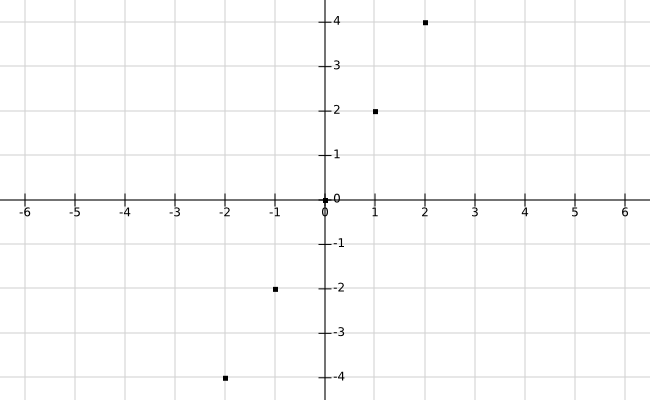
\includegraphics[scale=0.55]{image10.png}}
\caption{}
\label{}
\end{figure}
\newpage

\textbf{Kryssfråga 5:} Är signalen på bilden nedan diskret eller kontinuerlig?
\begin{enumerate}[label={\alph*)},font={\bfseries}]
\item Diskret
\item Kontinuerlig
\end{enumerate}

\begin{figure}[ht]
\centerline{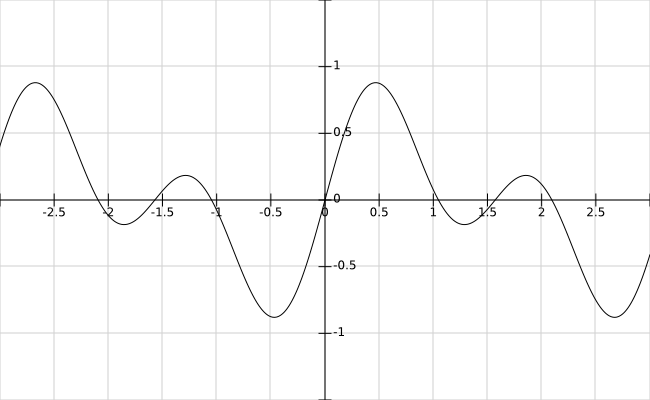
\includegraphics[scale=0.55]{image13.png}}
\caption{}
\label{}
\end{figure}

%TODO: I nuläget används både decimalkomma och decimalpunkt i texten. Problemet med decimalkomma är att det krockar med list-notation. Det är nog bäst att förklara detta och använda decimalpunkt trots att det i överigt är svensk text. Examples: 0,000001 ; 0,000002 ; 0,000003; 0,5; men också 0.5; 0.25
Det är möjligt, och rentav vanligt att approximera en kontinuerlig signal
med en diskret. Om man har väldigt små steg mellan värdena i den diskreta
approximationen, t.ex. $n={0.000001 ; 0.000002 ; 0.000003}$, kan man rentav få
en ganska bra approximation. I praktiken är detta faktiskt precis vad man gör när
man hanterar kontinuerliga signaler med datorer. En dator kan egentligen inte
hantera kontinuerliga signaler men den kan approximera dem med diskreta signaler
med väldigt små steg mellan värdena, vilket oftast är gott nog.
%*Bild på en kontinuerlig signal, t.ex. f(t)= sin(2t) och en diskret approximation av den.

\begin{figure}[ht]
\centerline{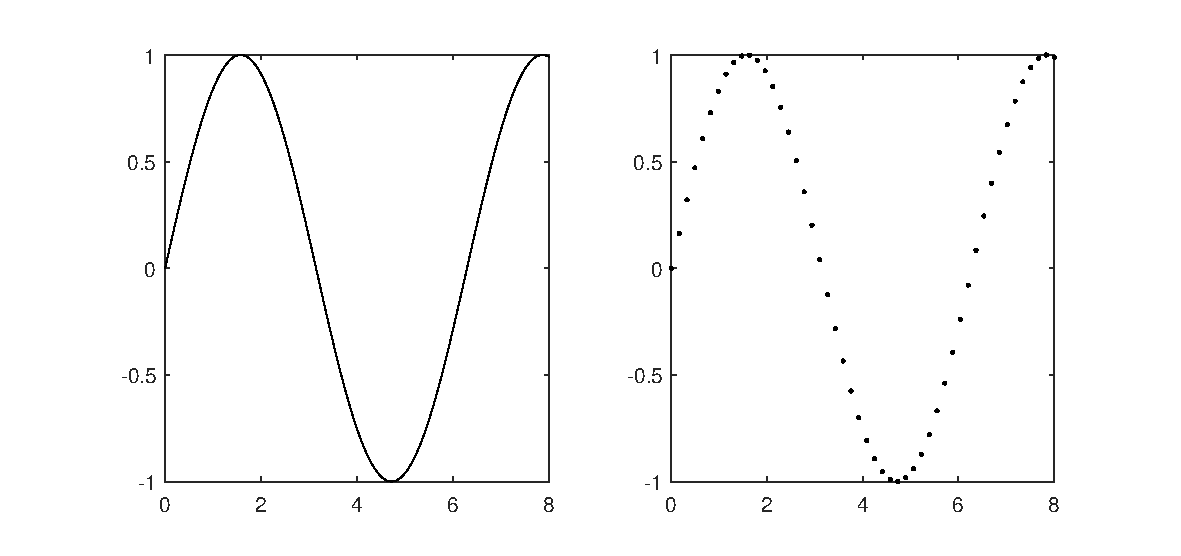
\includegraphics[scale=0.55]{images/diskretisering.eps}}
\caption{En kontinuerlig signal $f(t) = \sin(2 t)$ och dess diskreta approximation.}
\label{}
\end{figure}

\subsection{Periodiska Signaler}
En periodisk signal är precis som det låter, en signal som upprepar sig efter
ett visst tidsintervall, som kallas signalens period. Motsatsen till detta
kallas för en aperiodisk signal.
En signal kan vara aperiodisk om till exempel intervallet mellan varje
upprepning minskar eller om det aldrig upprepas alls.

Lite mer formellt definieras en periodisk signal så här:

$f(t) = f(t+T)$, för alla värden på t, där T är perioden

%Här ser du t.ex. en periodisk signal $f(t)=2 \sin(3 t)$, som har perioden $T=\frac{2\pi}{3}$. Notera att $f(t)=f(t+T)$ är sant, avsett vilken punkt t du tittar på. -flyttade in detta i caption.
\begin{figure}[ht]
\centerline{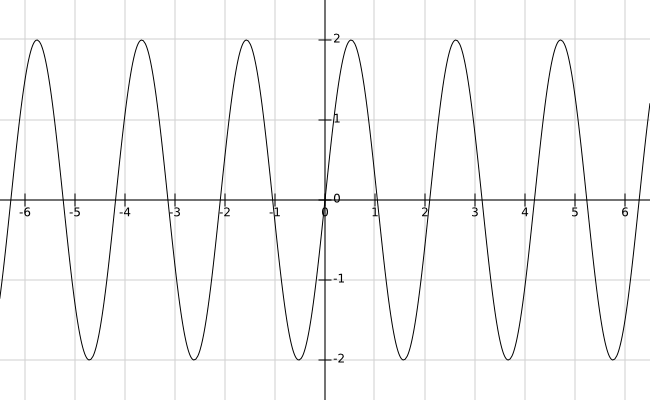
\includegraphics[scale=0.55]{image12.png}}
\caption{Här ser du t.ex. en periodisk signal $f(t)=2 \sin(3 t)$,
  som har perioden $T=\frac{2\pi}{3}$. Notera att $f(t)=f(t+T)$ är sant,
  avsett vilken punkt t du tittar på.}
\label{}
\end{figure}
\newpage
Övning 6: Här har du en nästan färdig funktion som undersöker om en
signal har en viss period. Fyll i det som ska stå i parentesen.
\begin{minted}{haskell}
contHasPeriod :: ContTimeFun ->
                 ContTime -> Double -> Bool
contHasPeriod signal step period =
        and $ map (...) [0, step .. period]
    where hasPeriod signal period t =
            signal t ~= signal (t+period)
\end{minted}

\textbf{Kryssfråga 6:} I bilden nedan ser du en funktion,
$f(t)=0.5\sin(2t)$. Vad har den för period?
\begin{enumerate}[label={\alph*)},font={\bfseries}]
    \item $\pi$
    \item 2 $\pi$
    \item 2
\end{enumerate}

\begin{figure}[ht]
\centerline{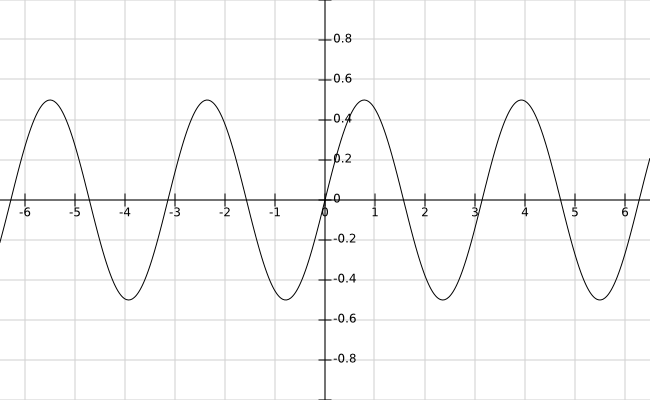
\includegraphics[scale=0.50]{image08.png}}
\caption{funktionen $f(t) = 0.5 \sin(2t)$}
\label{}
\end{figure}

\newpage

Kryssfråga 7: Här nedan ser vi en annan funktion, f(t)=3cos(0.25t).
Vad har den för period?
\begin{enumerate}[label={\alph*)},font={\bfseries}]
    \item $\frac{1}{4}\pi$
    \item $8\pi$
    \item $3\pi$
\end{enumerate}

\begin{figure}[ht]
\centerline{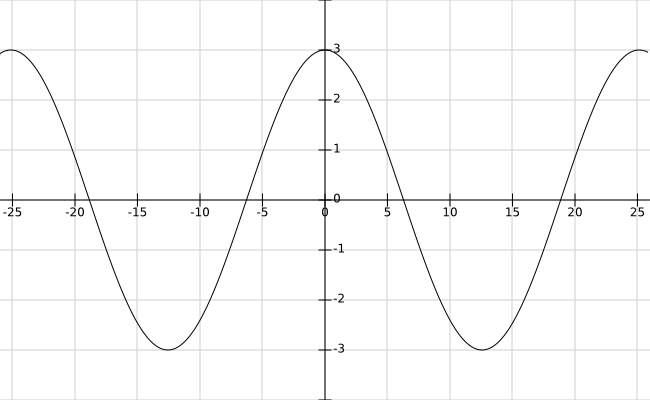
\includegraphics[scale=0.50]{image11.png}}
\caption{}
\label{}
\end{figure}

Vad har man då för nytta av att kunna avgöra om en signal är periodisk?
Jo, en periodisk signal kan utvecklas till en Fourier serie. Mer om detta i avsnitt 3.

\newpage

\subsection{Udda och Jämna Signaler}

Eftersom signaler kan betraktas som matematiska funktioner kan vi säga att vi
har udda och jämna signaler, precis som vi har jämna och udda funktioner.
En funktion kan vara jämn, udda eller inget utav dem.

En funktion f är jämn om $f(x)$ är samma som $f(-x)$.
I den vänstra bilden här nedan ser du ett exempel på en jämn funktion,
$f(x)=\cos(x)$. Notera att vilken punkt du än tittar på i figur 6a här
nedan så gäller alltid  $f(x) = f(-x)$.

En funktion f är udda om $f(-x)$ är samma som $-f(x)$. I den högra bilden
nedan ser du ett exempel på en udda funktion , $f(x)=sin(x)$.
Notera att vilken punkt du än tittar på i figur 6b här nedan så gäller
alltid $f(-x) = -f(x)$.

\begin{figure}[ht]
\centering
\begin{subfigure}{0.50\textwidth}
  \centering
  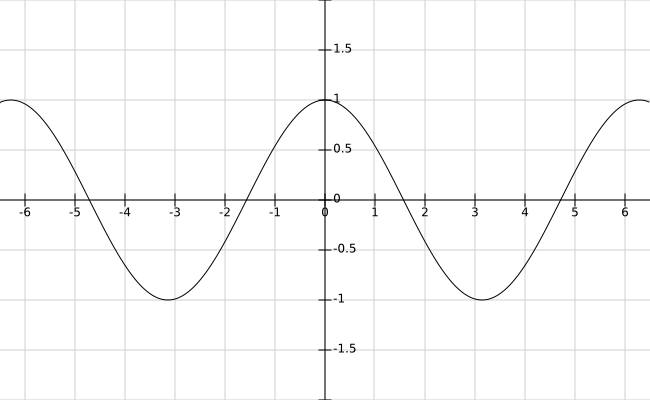
\includegraphics[width=0.90\linewidth]{image09.png}
  \caption{Jämn funktion}
  \label{}
\end{subfigure}%
\begin{subfigure}{0.50\textwidth}
  \centering
  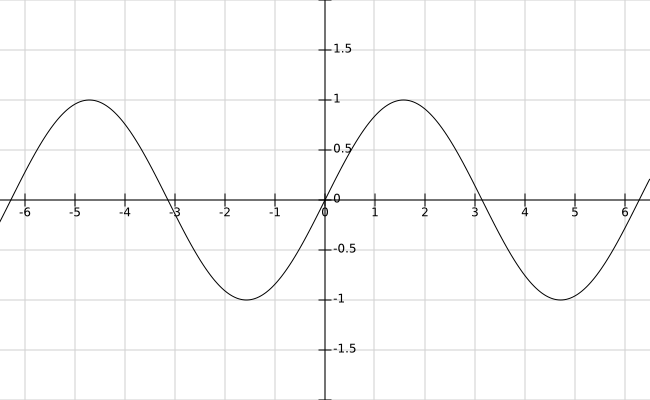
\includegraphics[width=0.90\linewidth]{image14.png}
  \caption{Udda funktion}
 \label{}
\end{subfigure}%
\caption{}
\label{}
\end{figure}



Alltså:

Jämn funktion:\hfill Udda funktion:

$ f(x)=f(-x)$ \hfill $f(-x)=-f(x) $

Varför är det då bra att veta om en signal är jämn eller udda?
Mer om det kommer i avsnittet om Fourierserier!

\newpage

\textbf{Kryssfråga 8:} Är funktionen $f(t)=0.5\sin(2t)$ här nedan jämn,
udda eller ingetdera?
\begin{enumerate}[label={\alph*)},font={\bfseries}]
    \item Jämn
    \item Udda
    \item Ingetdera
\end{enumerate}

\begin{figure}[ht]
\centerline{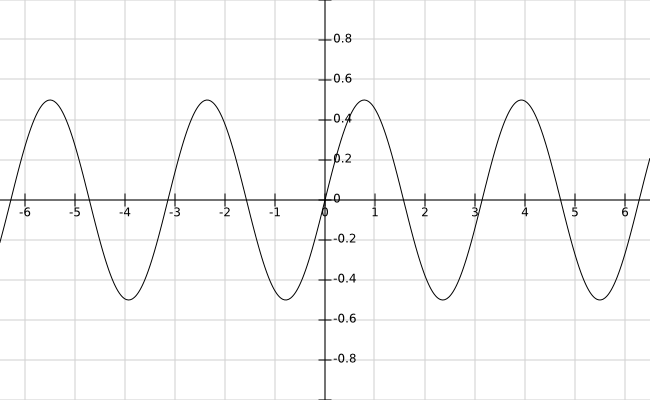
\includegraphics[scale=0.50]{image08.png}}
\caption{funktionen $f(t) = 0.5 \sin(2t)$}
\label{}
\end{figure}

\newpage

Kryssfråga 9: Är funktionen $f(t)=3\cos(0.25t)$ här nedan jämn, udda eller ingetdera?
\begin{enumerate}[label={\alph*)},font={\bfseries}]
    \item Jämn
    \item Udda
    \item Ingetdera
\end{enumerate}

\begin{figure}[ht]
\centerline{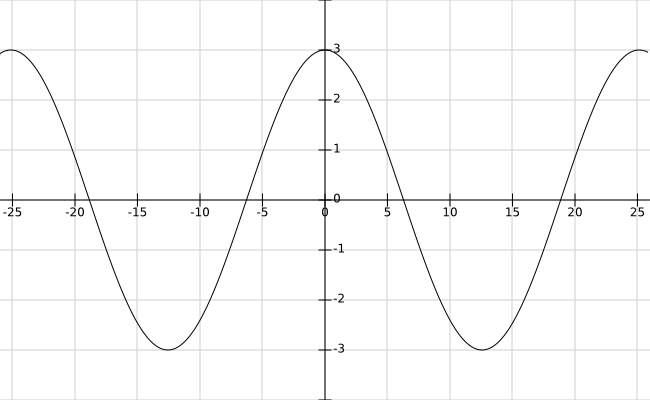
\includegraphics[scale=0.50]{image11.png}}
\caption{}
\label{}
\end{figure}

Då ska vi se hur man kan implementera det här! En funktion som avgör om en
signal är udda kan se ut så här:
\begin{minted}{haskell}
contIsOdd :: ContTimeFun -> ContTime -> Double -> Bool
contIsOdd signal step limit = and $ map testPair $ zip xs ys
    where testPair (a,b) = a ~= (-b)
          xs = map signal [0, step .. limit]
          ys = map signal [0,-step .. (-limit)]
\end{minted}

\textbf{Övning 7:} Implementera motsvarande funktion som undersöker
om en signal är jämn.

\textbf{Test:} Lös de två nedanstående uppgifter och kontrollera sedan svaret med
hjälp av programmet.

\textbf{Test 1:}
En signal har funktionen: $3*\sin(6t)$

Vad är signalens period?

Är signalen udda eller jämn?

\textbf{Test 2:}
En signal har funktionen: $\frac{1}{2} \cos(t)$

Vad är signalens period?

Är signalen udda eller jämn?

Testa gärna fler signaler!

\subsection{Enhetsimpulser}
En enhetsimpuls ser ut så här:


\begin{figure}[ht]
\centerline{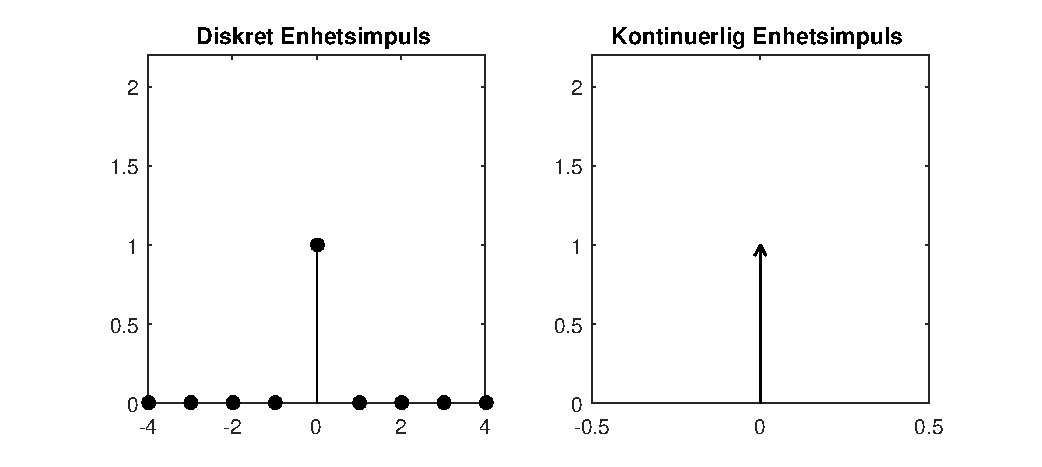
\includegraphics[scale=0.50]{delta.eps}}

%Tror var figurerna är skapade inte måste stå just här. Disclamer någon annanstans?
\caption{}
\label{}
\end{figure}

En enhetsimpuls kallas också för en dirac delta funktion och är i det
diskreta fallet definierad som:
$$
\delta[n]=
\begin{cases}
    1,\quad n = 0 \\
    0, \quad else
\end{cases}, n \in \mathbb{Z}
$$
Och i det kontinuerliga fallet är den definerad som:

$$\int_{-\infty}^{\infty} \delta(t) dt = 1 $$
där
$$
\delta(t)=
\begin{cases}
"\infty",\quad t = 0 \\
0, \quad else
\end{cases}, t\in \mathbb{R}
$$
Det vill säga, den är oändligt hög och oändligt smal då argumentet,
t.ex. t, är 0 och annars tar den värdet 0.
$$\int_{-\infty}^{\infty} \delta(t-\tau) f(t) dt = f(\tau) $$

Med andra ord, integralen av dessa blir värdet av integranden då
enhetsimpulsen antar värdet 1.

I praktiken kan en signal egentligen inte bestå av en riktig enhetsimpuls,
då en matematisk korrekt enhetsimpuls bara är definierad inuti en intergral.
Men, precis som med mycket annat, kan man approximera en enhetsimpuls med något
som är nära nog en riktig enhetsimpuls.

\textbf{Övning 8:} Här får du ett kodskelett till en definition av en diskret
enhetsimpuls med DSL. Fyll i det som saknas.
\begin{minted}{haskell}
discImpulse :: DiscTimeFun
discImpulse n | ...
              | otherwise = ...
\end{minted}

\subsection{Enhessteg}
Ett enhetssteg ser ut så här:

\begin{figure}[h]
\centerline{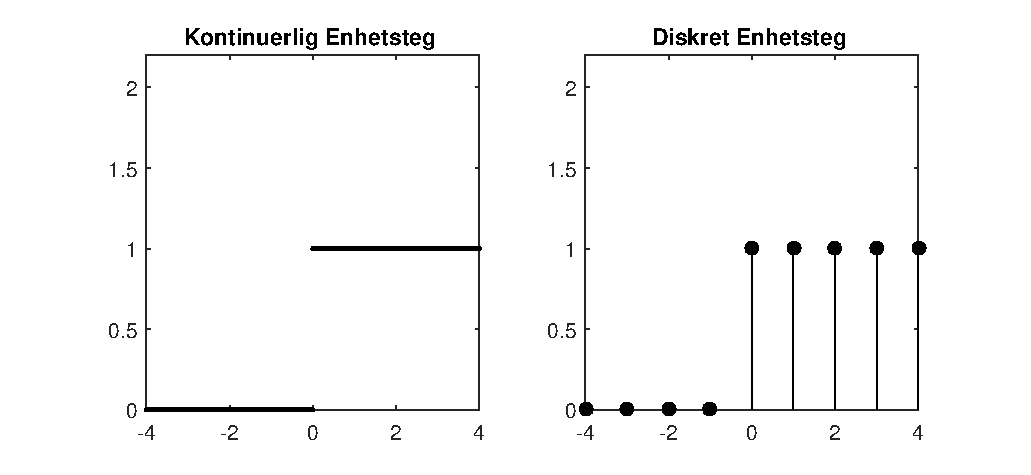
\includegraphics[scale=0.50]{heavy.eps}}
\caption{}
\label{}
\end{figure}

En enhetstegsfunktion kallas även för en heavyside function och är i det
diskreta fallet definierad som:
$$
u[t] =
\begin{cases}
0, \quad n < 0 \\
1, \quad n \geq 0
\end{cases}
$$

Och i det kontinuerliga fallet definerad som:
$$
u(t) =
\begin{cases}
0, \quad t < 0 \\
1, \quad t \geq 0
\end{cases}
$$
Det vill säga om tiden eller argumentet inuti funktionen är större eller lika
med noll, antar funktionen $u(t)$ värdet 1, annars är den 0.
Denna uppkommer oftast multiplicerad med en annan funktion som
$u(t-\tau) f(t)$. Det kan då tolkas som att $f(t)$ finns efter en tidpunkt $t = \tau$.

\begin{figure}[ht]
\centerline{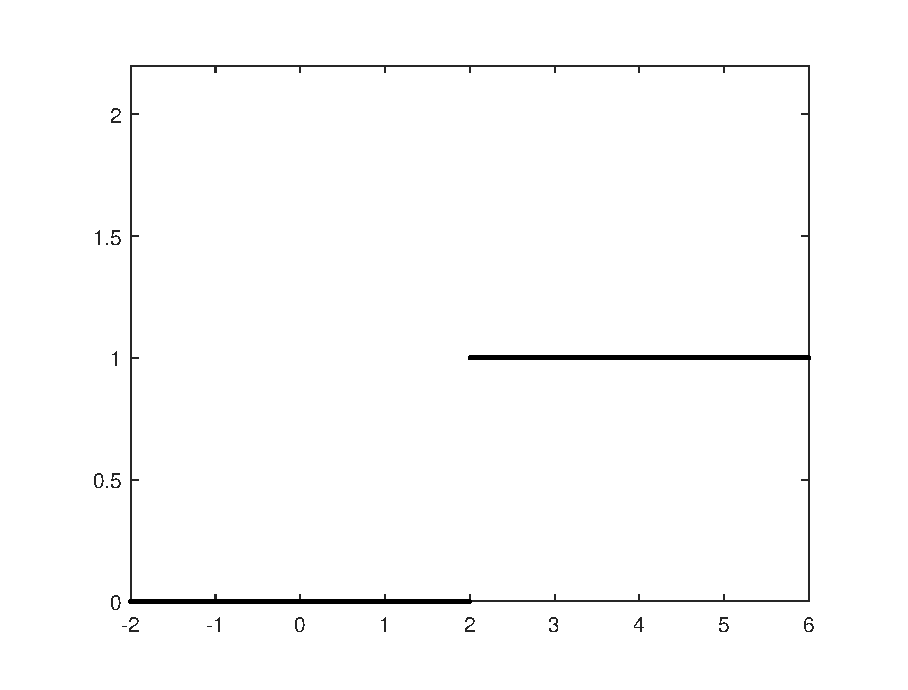
\includegraphics[scale=0.50]{shiftedHeavy.eps}}
\caption{Ett tidskiftad kontinuerlig enhetsteg med $\tau = 2$.}
\label{}
\end{figure}

\textbf{Övning 9:} Här får du ett kodskelett till en definition av ett
diskret enhetssteg med DSL. Fyll i det som saknas.
\begin{minted}{haskell}
discStep :: DiscTimeFun
discStep n | ...
           | ...
\end{minted}
\newpage
\subsection{Sammanfattning}
Gratulerar! Du har nu lärt dig följande:
\begin{itemize}
\item Vad komplexa tal är
\item Hur man gör några vanliga beräkningar med komplexa tal
\item Hur man implementerar komplexa tal med funktionell programmering i en DSL
\item Hur man implementerar vanliga beräkningar med komplexa tal med
  funktionell programmering i en DSL
\item Vad Eulers formel är
\item Hur man kan skriva om trigonometriska och komplexa uttryck med Eulers formel
\item Hur man implementerar Eulers formel med funktionell programmering i en DSL
\item Vad diskreta och kontinuerliga signaler är
\item Vad periodiska signaler är
\item Vad udda och jämna signaler är
\item Hur man implementerar funktioner för jämna och udda funktioner med DSL.
\item Vad enhetssteg och enhetsimpulser är.
\item Hur man implementerar diskreta enhetssteg och enhetsimpulser med DSL.
\end{itemize}

Bilderna i detta kapitel är gjorda i:
\begin{itemize}
\item MATLAB: Figur 4, 11, 12 och 13
\item FOOPLOT: Figur 1, 2, 3, 5, 6, 7, 8, 9 och 10
\end{itemize}

\newpage
\section{Lösningar}

\textbf{Kryssfråga 1:} b) 10

\textbf{Kryssfråga 2:} b) 65

\textbf{Övning 1:}
\begin{minted}{haskell}
imPart :: Complex -> Double
imPart (Complex c) = snd c
\end{minted}
\textbf{Övning 2:}
\begin{minted}{haskell}
printComplex :: Complex -> String
printComplex z
  | r == 0 = show im ++ "j"
  | im == 0 = show r
  | otherwise = show r ++ " + " ++ show im ++ "j"
    where im = imPart z
          r = realPart z
\end{minted}
\textbf{Övning 3:}
\begin{minted}{haskell}
instance Num Complex where
    z + w           = Complex (realPart z +
                        realPart w, imPart z + imPart w)
\end{minted}

\textbf{Övning 4:}
\begin{minted}{haskell}
   negate z        = Complex (negate $ realPart z, negate $ imPart z)
\end{minted}

\textbf{Övning 5:}
\begin{minted}{haskell}
    abs z           = Complex (hyp, 0)
        where hyp   = sqrt (r*r + im*im)
              r     = realPart z
              im    = imPart z
\end{minted}
\textbf{Kryssfråga 3:} b) $\cos(3t) + j\sin(3t)$

\textbf{Kryssfråga 4:} c) $e^{j4} + 5$

\textbf{Kryssfråga 5:} b) Kontinuerlig
\newline
\textbf{Övning 6:}
\begin{minted}{haskell}
contHasPeriod :: ContTimeFun -> ContTime ->
                                        Double -> Bool
contHasPeriod signal step period =
        and $ map (hasPeriod signal period)
                                [0, step .. period]
    where hasPeriod signal period t =
                            signal t ~= signal (t+period)
\end{minted}

\textbf{Kryssfråga 6:} a) $\pi$

\textbf{Kryssfråga 7:} b) $8\pi$

\textbf{Kryssfråga 8:} b) Udda

\textbf{Kryssfråga 9:} a) Jämn

\textbf{Övning 7:}
\begin{minted}{haskell}
contIsEven :: ContTimeFun -> ContTime -> Double -> Bool
contIsEven signal step limit = and $ map testPair $ zip xs ys
    where testPair (a,b) = a ~= b
          xs = map signal [0, step .. limit]
          ys = map signal [0,-step .. (-limit)]
\end{minted}
\textbf{Övning 8:}
\begin{minted}{haskell}
discImpulse :: DiscTimeFun
discImpulse n | n == 0 = 1
              | otherwise = 0
\end{minted}
\textbf{Övning 9:}
\begin{minted}{haskell}
discStep :: DiscTimeFun
discStep n | n < 0 = 0
           | otherwise = 1
\end{minted}

\end{document}
